

\documentclass["../Applied_probabillity _and_statistics_lab_KTU.tex"]{subfiles}
 
 \begin{document}


\section*{What we will learn}
In this experiment we will try to  learn the preliminaries of R along with methods of visualizing data in R

Tables, charts and plots. Visualizing Measures of Central Tendency, Variation,
and Shape. Box plots, Pareto diagrams. How to find the mean median standard
deviation and quantiles of a set of observations.




\section{Introduction to R}
To be written 
\subsection{Installing R }
  Platforms Window and linux
  
  Installing R on a Windows PC

To install R on your Windows computer, follow these steps:
\begin{enumerate}


  \item   Go to http://ftp.heanet.ie/mirrors/cran.r-project.org.
    \item Under “Download and Install R”, click on the “Windows” link.
    \item Under “Subdirectories”, click on the “base” link.
    \item On the next page, you should see a link saying something like “Download R 2.10.1 for Windows” (or R X.X.X, where X.X.X gives the version of R, eg. R 2.11.1). Click on this link.
    \item You may be asked if you want to save or run a file “R-2.10.1-win32.exe”. Choose “Save” and save the file on the Desktop. Then double-click on the icon for the file to run it.
    \item You will be asked what language to install it in - choose English.
    \item The R Setup Wizard will appear in a window. Click “Next” at the bottom of the R Setup wizard window.
    \item The next page says “Information” at the top. Click “Next” again.
    \item The next page says “Information” at the top. Click “Next” again.
    \item The next page says “Select Destination Location” at the top. By default, it will suggest to install R in “C:\\Program Files” on your computer.
    \item Click “Next” at the bottom of the R Setup wizard window.
    \item The next page says “Select components” at the top. Click “Next” again.
    \item The next page says “Startup options” at the top. Click “Next” again.
    \item The next page says “Select start menu folder” at the top. Click “Next” again.
    \item The next page says “Select additional tasks” at the top. Click “Next” again.
    \item R should now be installed. This will take about a minute. When R has finished, you will see “Completing the R for Windows Setup Wizard” appear. Click “Finish”.
  \item   To start R, you can either follow step 18, or 19:
    \item Check if there is an “R” icon on the desktop of the computer that you are using. If so, double-click on the “R” icon to start R. If you cannot find an “R” icon, try step 19 instead.
    \item Click on the “Start” button at the bottom left of your computer screen, and then choose “All programs”, and start R by selecting “R” (or R X.X.X, where X.X.X gives the version of R, eg. R 2.10.0) from the menu of programs.
    \item The R console (a rectangle) should pop up:

  
  \end{enumerate}
  \begin{figure}
 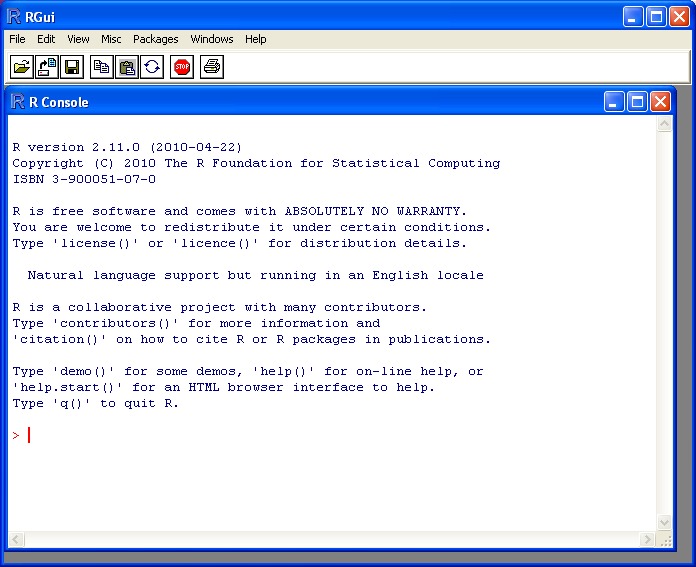
\includegraphics[scale=.4]{chapters/images/console.png}
 \label{console_windows}
 \end{figure} 
  
  
  
\subsection{Installing R studio}
\begin{enumerate}
 \item    Go to RStudio IDE download page.
   \item   Click Download RStudio Desktop.
  \item    Then click for the download link recommended for your system.
  \item    Run the downloaded file (double click the file) to start the setup wizard.
  \item    Click “Next” until “Finish”
\end{enumerate}
     
 \section{R fundamentals}
 
This is a review of R fundamentals. No details are covered. It is assumed that the participant is familiar with programming.
\subsection{Basic Math operations in R}
Type the following  on > prompt and see the results. 
 \begin{lstlisting}[language=R]
1 + 1
5 - 3
3 * 3
4 / 5
4 ^ 2   # Exponetiation
5 %% 2   # Modulus
5 %/% 2  # integer division


\end{lstlisting}

\subsection{Variables and assignment in R}
 There is no  need to declare variables in advance. Rules for variable names are almost similar to those in C programming language. There are two assignment : + and <-.  The preferred assignment operator is <- . 
 Try the following.
  \begin{lstlisting}[language=R]
x=20  # assign x=20
y<-3  # assign y =3
x     # Display x
y     # Display y
x=y
x
y<-x*10

\end{lstlisting}

A variable can be removed using rm() function.

 \begin{lstlisting}[language=R]
 rm()  # remove x 
 x     # try printing x after removal
\end{lstlisting}

\subsection{R Data Types}
R has a wide variety of data types including scalars, vectors (numerical, character, logical), matrices, data frames, and lists. Let us quickly review them.
\begin{lstlisting}[language=R]
# An integer can be assigned to a variable by suffixing L
x=5L
class(x)   # This prints the data type of x
 
# numeric 
y=5.3
class(y)

# Character string
y=" hello"
class(y)

# date
date=as.Date("2016-10-16")
date

\end{lstlisting}
 
 \subsection{Logical operators}
 Similar to C > < <= >= == !=
 
\begin{lstlisting}[language=R]
 5>6

\end{lstlisting}
\subsection{Control statements}
 \subsubsection*{if-else}
    \begin{lstlisting}[language=R]
 x <- 5
if(x > 0){
   print("Positive number")
}

\end{lstlisting}
 \subsubsection*{ifelse}
 
    \begin{lstlisting}[language=R]
 a = c(5,7,2,9)  # a is a vector. The function c creates vector a
 a   #print a  
 ifelse(a %% 2 == 0,"even","odd")

\end{lstlisting}

 \subsubsection*{for loops}
    \begin{lstlisting}[language=R]
 x <- c(2,5,3,9,8,11,6) # x is  a vactor 
count <- 0
for (val in x) {
    if(val %% 2 == 0)  count = count+1
}
print(count)

\end{lstlisting}
 \subsubsection*{while loops}
    \begin{lstlisting}[language=R]
 i <- 1

while (i < 6) {
   print(i)
   i = i+1
}

\end{lstlisting}
 
 \section{R data structures}
 

Here we will review and learn basic data structures commonly used in R.
\subsection{Vector}


A fundamental R data structure is the vector, which stores an ordered set of values called elements. A vector can contain any number of elements. However, all the elements must be of the same type; for instance, a vector cannot contain both numbers and text.

You can build a vector as below using the c() function. c functions combines several entities of to a vector.
   
    \begin{lstlisting}[language=R]
 
state<- c("Kerala","Tamil Nadu"," Maharashtra")

\end{lstlisting}
 
 A vector can be printed by typing its name at the R prompt.
    \begin{lstlisting}[language=R]
state
\end{lstlisting}
 Let us create several vectors.

    \begin{lstlisting}[language=R]
temperature <- c(98.1, 98.6, 101.4)
capital <- c("tvm","chennai","mumbai")
drought <- c(FALSE, FALSE, TRUE)
\end{lstlisting}
 Let us print them.

\begin{lstlisting}[language=R]
state
temperature
capital
drought

\end{lstlisting}
 

You can access individual elements using square brackets.
\begin{lstlisting}[language=R]
 temperature[2]
\end{lstlisting}



You can create a vector containing a sequence of numbers using :

\begin{lstlisting}[language=R]
 x=10:50
x
x[3]
y=-2:5
z=10:1
y
z
\end{lstlisting}

\subsubsection{Vector Operations}

\begin{lstlisting}[language=R]

x*3 

x/4
x+2
sqrt(x)
y=1/x
y
x=1:10
y=10:1
x+y
x-y
x*y
x/y
length(x)
m=c(1,2)
x
x+m
x<5
\end{lstlisting}

\subsection{Factors}
Factor is a data structure used for fields that takes only predefined, finite number of values (categorical data). For example, a data field such as marital status may contain only values from single, married, separated, divorced, or widowed. In such case, we know the possible values beforehand and these predefined, distinct values are called levels
\begin{lstlisting}[language=R]
status <- factor(c("single","married","married","single"));
status
\end{lstlisting}

\subsection{Lists}
Let us create and print  a list.
\begin{lstlisting}[language=R]
 n = c(2, 3, 5) 
 s = c("aa", "bb", "cc", "dd", "ee") 
 b = c(TRUE, FALSE, TRUE, FALSE, FALSE) 
 x = list(n, s, b, 3)   # x contains copies of n, s, b

x
\end{lstlisting}
Display list elements.
\begin{lstlisting}[language=R]
x[2]
x[[2]]
x[[2]][1]
\end{lstlisting}


\subsection{Data Frames}

A data frame is used for storing data tables. It is a list of vectors of equal length. For example, the following variable df is a data frame containing three vectors n, s, b.
\begin{lstlisting}[language=R]
 n = c(2, 3, 5) 
 s = c("aa", "bb", "cc") 
 b = c(TRUE, FALSE, TRUE) 
 df = data.frame(n, s, b)  
 
 # print the data frame df
 df
\end{lstlisting}


Accessing rows and columns of data frame.
\begin{lstlisting}[language=R]
df[1]
df[[1]]
df$n
df[2,2]

\end{lstlisting}
\subsubsection{Examining some built in data frames.}
There are several built in data frames you can use. mtcars is a simple frame about car parameters.
\begin{lstlisting}[language=R]
 mtcars
help(mtcars) # read the documentation.
\end{lstlisting}
 Let us experiment with this data set.
 
 \begin{lstlisting}[language=R]
mtcars[1, 2]

mtcars["Mazda RX4", "cyl"] 
mtcars["Mazda RX4",]
nrow(mtcars) 

ncol(mtcars)  
head(mtcars)
mtcars[[9]] 

mtcars[["am"]] 
mtcars$am
mtcars[1] 

mtcars["mpg"]
mtcars[c("mpg", "hp")]
mtcars[24,] 

mtcars[c(3, 24),] 
mtcars["Camaro Z28",] 
mtcars[c("Datsun 710", "Camaro Z28"),]
\end{lstlisting}

\subsection{Exercises}
  Examine iris data set.
  
\subsection{Importing Data}  
Download the iris data set from . 
Read the background information from wikipedia.

Data can be stored in a comma separated value format Common extension is .csv. You can read a csv file as below. It is assumed that the file is in your current directory. If you get an error here most probably you are in wrong directory or the data file is missing. Please download the data file and place it in your current directory. 

\begin{lstlisting}[language=R]
 mydata = read.csv("iris.csv")  # read csv file. Make sure that you have the csv file
\end{lstlisting}
 If you get an error, please try out the following commands. 
 \begin{lstlisting}[language=R]
 

getwd()  # This command prints your current directory

setwd("/home//sunil")   # use this commnad to set the direcotry.


mydata = read.csv("iris.csv")  # read csv file

mydata
str(mydata  ) # display the structure of mydata variable

\end{lstlisting}
 
\subsection{
Find out statistics of your data.}

\begin{lstlisting}[language=R]
 mean(mtcars$mpg)
median(mtcars$mpg)
sd(mtcars$mpg)
summary(mtcars)



range(mtcars$mpg)
diff(range(mtcars$mpg))


IQR(mtcars$mpg) # I am not explaining this. Find out from documentation.:D
\end{lstlisting}

Repeat the above for iris data set.

 \section{Plotting in R}
\subsection{Box Plots}
Boxplots are a measure of how well distributed is the data in a data set. It divides the data set into three quartiles. This graph represents the minimum, maximum, median, first quartile and third quartile in the data set. It is also useful in comparing the distribution of data across data sets by drawing boxplots for each of them. 
\begin{lstlisting}[language=R]
 

boxplot(mpg ~ cyl, data = mtcars, xlab = "Number of Cylinders",
   ylab = "Miles Per Gallon", main = "Mileage Data")


\end{lstlisting}

\subsection{Histograms}
\begin{lstlisting}[language=R]
 # Create data for the graph.
v <-  c(9,13,21,8,36,22,12,41,31,33,19)
hist(v,xlab = "Weight",col = "yellow",border = "blue")


hist(mtcars$mpg, main = "Histogram of  miles per gallon",
xlab = "mpg")

\end{lstlisting}
\subsection{Line graph}
\begin{lstlisting}[language=R]
 v <- c(7,12,28,3,41)
plot(v,type = "o") 
 
 

# multiple lines
v <- c(7,12,28,3,41)
t <- c(14,7,6,19,3)
plot(v,type = "o",col = "red", xlab = "Month", ylab = "Rain fall", 
   main = "Rain fall chart")
lines(t, type = "o", col = "blue")


\end{lstlisting
\subsection{Scatter plots}

\begin{lstlisting}[language=R]
 plot(x = mtcars$mpg,y = mtcars$cyl)
 help (plot )
 plot(x = mtcars$mpg, y = mtcars$hp,
main = "Scatterplot of mpg vs. hp",
xlab = "mpg",
ylab = "hp")


pairs(~wt+mpg+disp+cyl,data = mtcars,
   main = "Scatterplot Matrix")


\end{lstlisting}
\end{document}


